% Dit werk is gelicenseerd onder de licentie Creative Commons Naamsvermelding-GelijkDelen 4.0 Internationaal. Ga naar http://creativecommons.org/licenses/by-sa/4.0/ om een kopie van de licentie te kunnen lezen.
\documentclass[t]{beamer}

\usepackage{amsmath,amsthm}             % Uitgebreide wiskundige mogelijkheden
\usepackage{xcolor}						% Om kleuren te gebruiken

%%%%%%%%%%%%%%%%%%%%%%%%%%%%%%%%%%%%%%%%%%%%%%%%%%%%%%%%%%%%
% Nieuwe commandos
%%%%%%%%%%%%%%%%%%%%%%%%%%%%%%%%%%%%%%%%%%%%%%%%%%%%%%%%%%%%

% De differentiaal operator
\newcommand{\diff}{\ensuremath{\mathrm{d}}}
\newcommand{\subsdiff}{\ensuremath{\mathrm{D}}}
\newcommand{\vardiff}{\ensuremath{\mathrm{\delta}}}

% Super en subscript
\newcommand{\supsc}[1]{\ensuremath{^{\text{#1}}}}   % Superscript in tekst
\newcommand{\subsc}[1]{\ensuremath{_{\text{#1}}}}   % Subscript in tekst

% Vectoren en matrices
\newcommand{\vt}[1]{\ensuremath{\boldsymbol{#1}}} % vector in juiste lettertype
\newcommand{\mx}[1]{\ensuremath{\mathsf{#1}}}	  % matrix in juiste lettertype

% Nieuw commando om iets te benadrukken en tegelijkertijd in de index te steken.
\newcommand{\begrip}[1]{\index{#1}\textbf{#1}\xspace}

% Graden celcius
\newcommand{\degC}{\ensuremath{^\circ \mathrm{C}}}
% graden
\renewcommand{\deg}{\ensuremath{^\circ}}

% unit
\newcommand{\unit}[1]{\ensuremath{\mathrm {#1}}}


% underlinered
\newcommand{\underlinered}[1]{\color{red}\underline{{\color{black}#1}}\color{black}}
%%%%%%%%%%%%%%%%%%%%%%%%%%%%%%
% Packages
%%%%%%%%%%%%%%%%%%%%%%%%%%%%%%

%\usepackage{geometry}              	% 
\usepackage[dutch]{babel}               % Voor nederlandstalige hyphenatie (woordsplitsing)
\uselanguage{dutch}
\languagepath{dutch}
\usepackage{amsmath,amsthm}             % Uitgebreide wiskundige mogelijkheden
\usepackage{url}                        % Om url's te verwerken
\usepackage{graphicx,subfigure}         % Om figuren te kunnen verwerken
\usepackage[utf8]{inputenc}             % Om niet ascii karakters rechtstreeks te kunnen typen
\usepackage[section]{placeins}			% Om ervoor te zorgen dat floats binnen dezelfde section blijven
\usepackage{multicol}
\usepackage[absolute,overlay]{textpos}

%%%%%%%%%%%%%%%%%%%%%%%%%%%%%%
% Layout
%%%%%%%%%%%%%%%%%%%%%%%%%%%%%%
\usetheme{Frankfurt}
\usefonttheme[onlymath]{serif}
\AtBeginSection[]
{
  \begin{frame}
    \frametitle{Inhoud}
    \tableofcontents[currentsection]
  \end{frame}
}

\setbeamertemplate{navigation symbols}{}
\setbeamertemplate{footline}[page number]

%%%%%%%%%%%%%%%%%%%%%%%%%%%%%%
% Title
%%%%%%%%%%%%%%%%%%%%%%%%%%%%%%
\title{Fluïdummechanica}
\author{Brecht Baeten\inst{1}}
\institute{
	\inst{1}%
  		KU Leuven, Technologie campus Diepenbeek,\\ e-mail: brecht.baeten@kuleuven.be
}
\date{\today}
%%%%%%%%%%%%%%%%%%%%%%%%%%%%%%
% Omgevingen
%%%%%%%%%%%%%%%%%%%%%%%%%%%%%%


\subtitle{Gelijkvormigheid en dimensieloze getallen}

\begin{document}

	\frame{\titlepage}
	\section{Inleiding}
	\begin{frame}
		\frametitle{Voorbeeld}
		\center
    	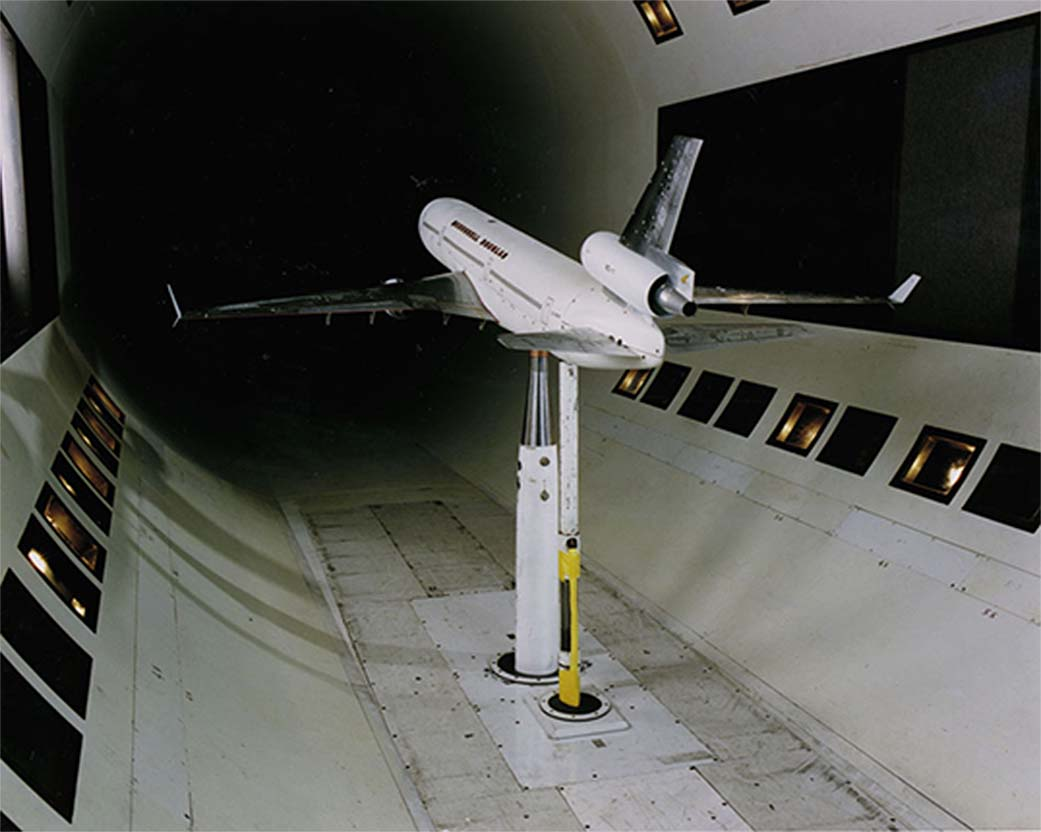
\includegraphics[height=0.8\textheight]{../fig/gelijkvormigheid/airplane_in_windtunnel.jpg}\\
		\footnotesize{Bron: http://www.nasa.gov/}
  	\end{frame}
  	\begin{frame}
		\frametitle{Voorbeeld}
		\center
    	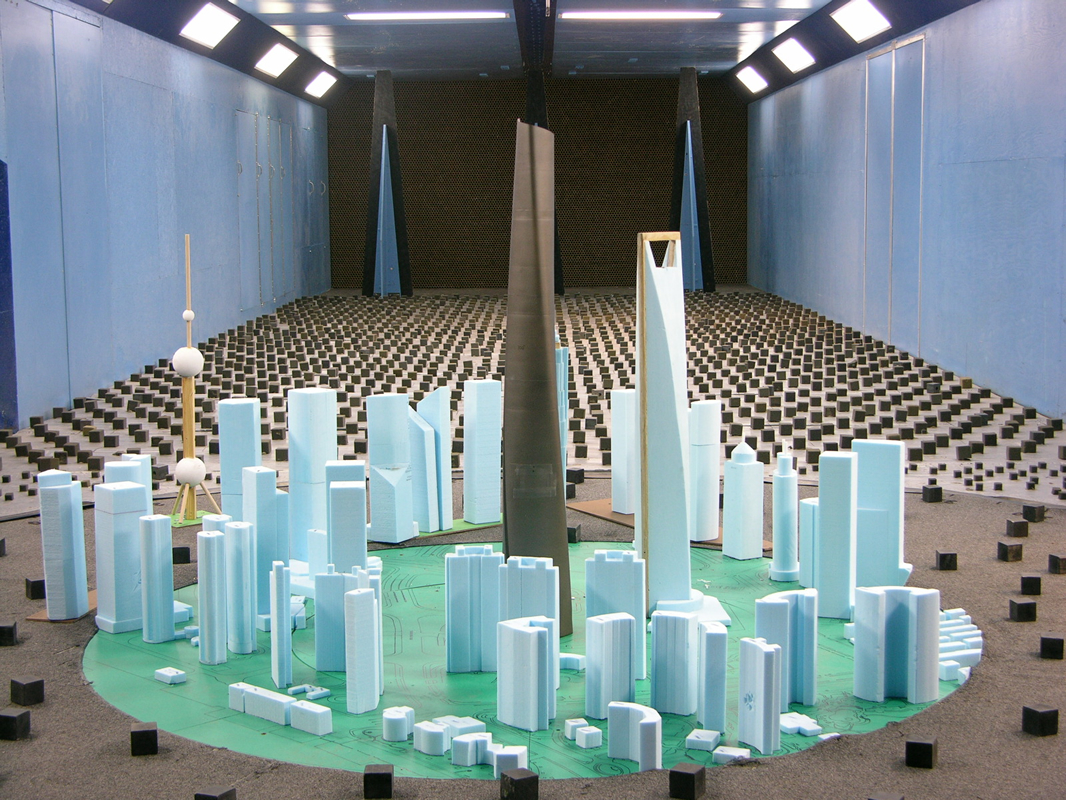
\includegraphics[height=0.8\textheight]{../fig/gelijkvormigheid/shanghai_tower_windtunnel.jpg}\\
		\footnotesize{Bron: http://www.autodesk.com/}
  	\end{frame}
%%%%%%%%%%%%%%%%%%%%%%%%%%%%%%%%%%%%%%%%%%%%%%%%%%%%%%%%%%%%%%%%%%%%%%%%%%%
	\section{Gelijkvormigheid}	
  	\begin{frame}
		\frametitle{Wat is gelijkvormigheid?}

		\centering
		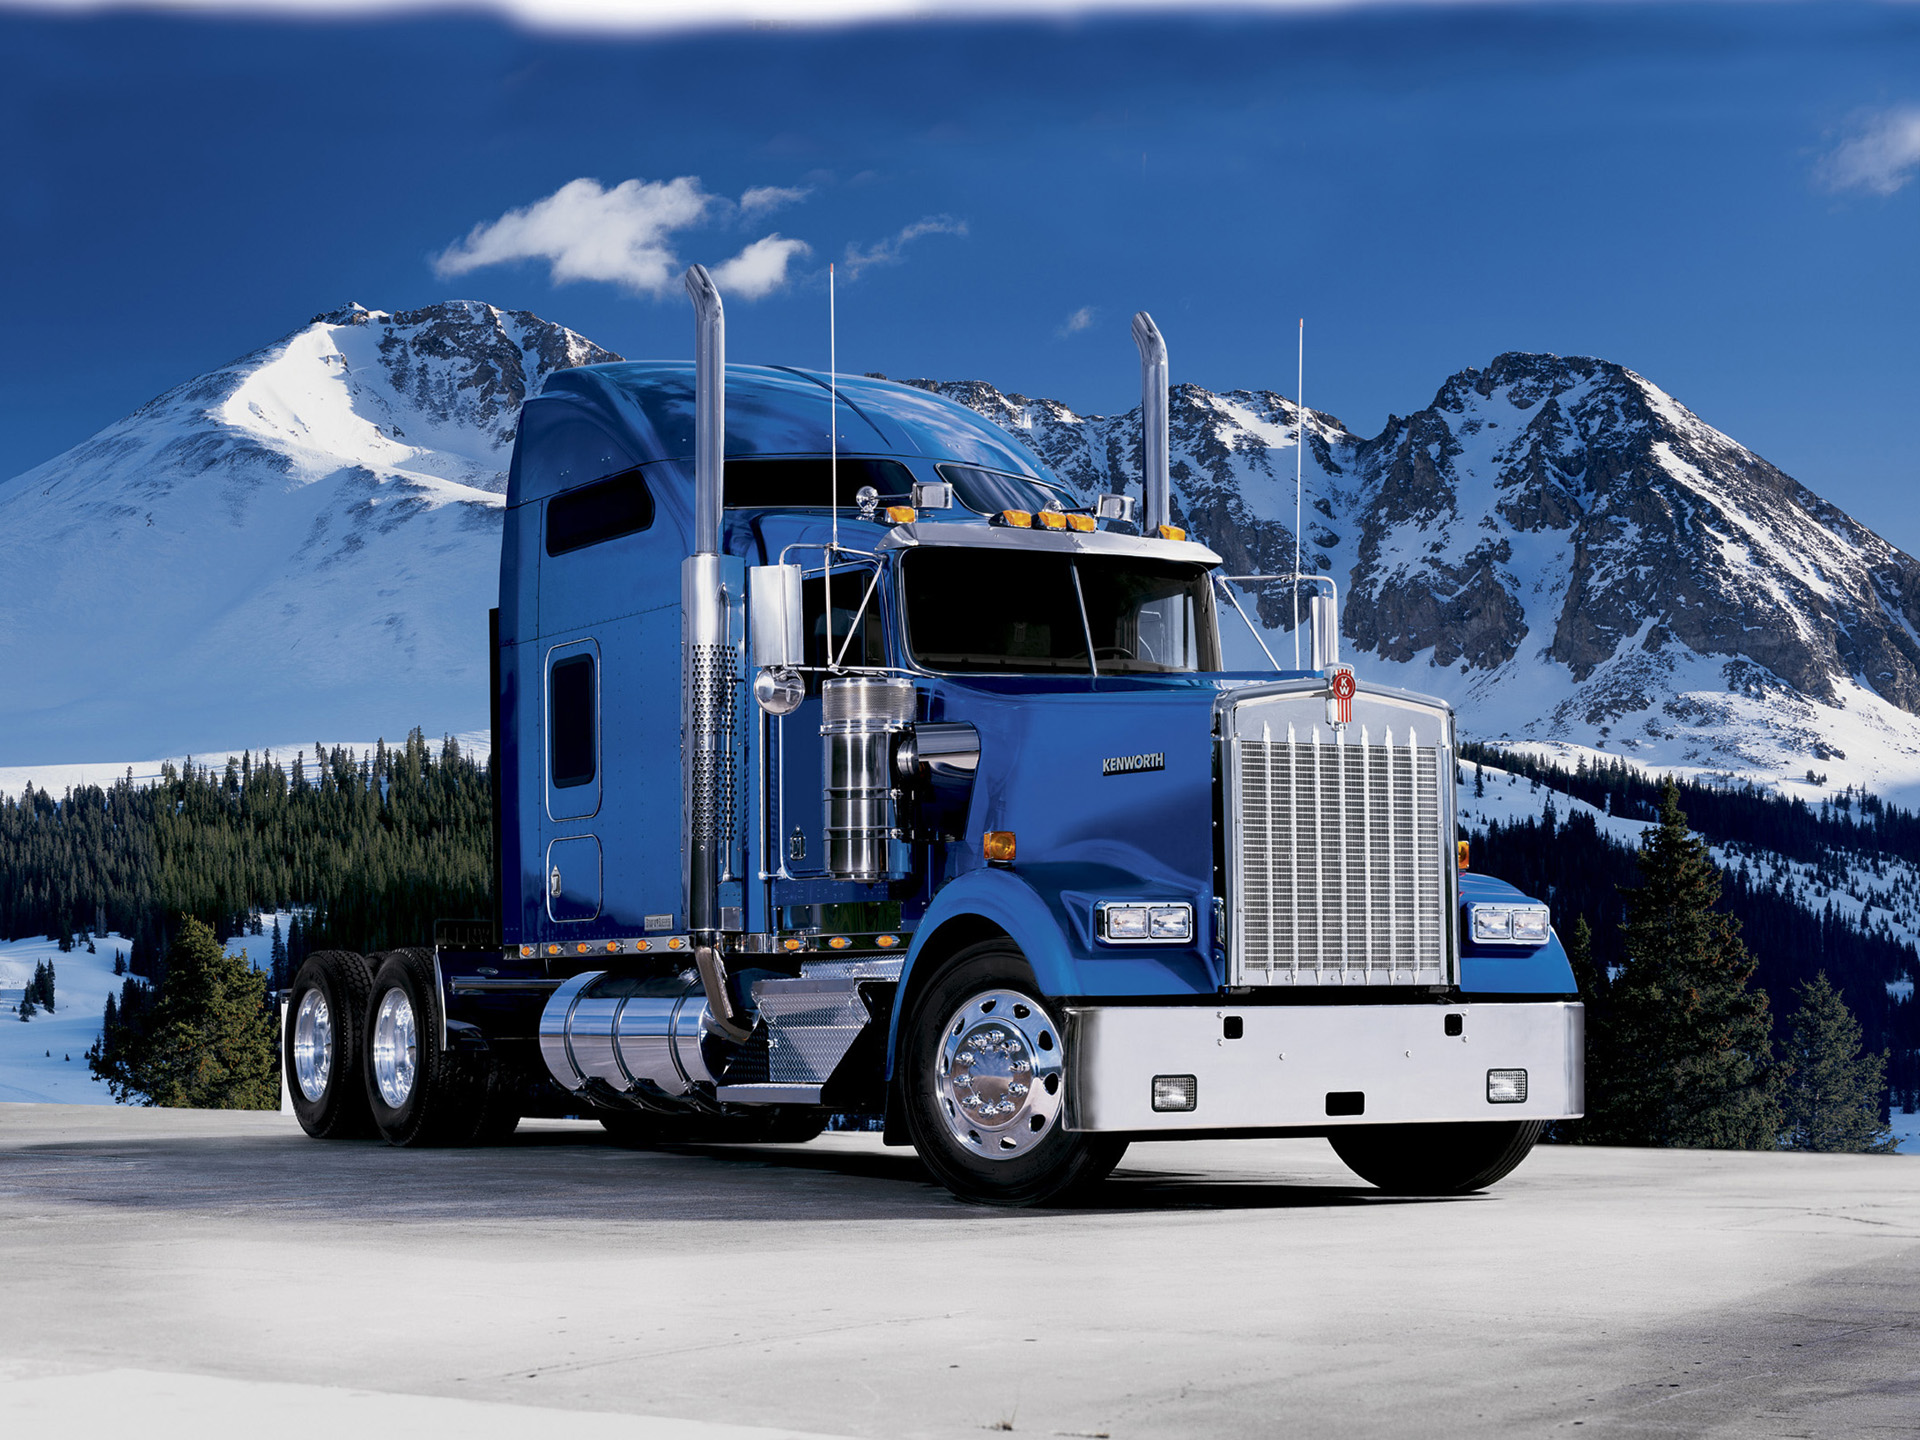
\includegraphics[height=0.8\textheight]{../fig/gelijkvormigheid/6931636-kenworth-w900-wallpaper-hd.jpg}\\
		\footnotesize{Bron: http://7-themes.com/}
  	\end{frame}
%%%%%%%%%%%%%%%%%%%%%%%%%%%%%%%%%%%%%%%%%%%%%%%%%%%%%%%%%%%%%%%%%%%%%%%%%%%
  	\begin{frame}
		\frametitle{Wat is gelijkvormigheid?}
		
		\begin{itemize}
			\item<2-3> Gelijke verhoudingen van afstanden
			\item<3-3> Gelijke verhoudingen van snelheden
		\end{itemize}

        \vspace{0.1cm}
               
        \only<2>{
        	\center
            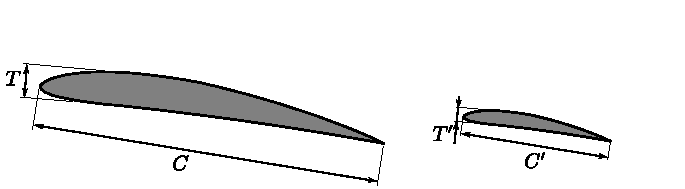
\includegraphics[width=11cm]{../fig/gelijkvormigheid/Gelijkvormigheid_geometrisch}
		}
        \only<3>{
        	\center
            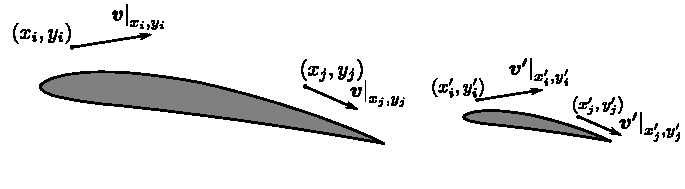
\includegraphics[width=11cm]{../fig/gelijkvormigheid/Gelijkvormigheid_kinematisch}
        }
		
  	\end{frame}
%%%%%%%%%%%%%%%%%%%%%%%%%%%%%%%%%%%%%%%%%%%%%%%%%%%%%%%%%%%%%%%%%%%%%%%%%%%
	\section{Dimensieloze getallen}	
  	\begin{frame}
		\frametitle{Het dimensieloos maken van de bewegingsvergelijking}
		\begin{equation*}
			\rho \frac{\partial v}{\partial t} + \rho v \frac{\partial v}{\partial s} = -\frac{\partial p}{\partial s} + \rho g_s + \mu \frac{\partial^2 v}{\partial s^2}
		\end{equation*}
		\pause
		\hspace{5cm} $\Downarrow \quad  \begin{array}{lcl}	s &=& s^* D_{\text{ref}} \\ v &=& v^* v_{\text{ref}}  \\ t &=& t^* t_{\text{ref}} \\ p &=& p^* p_{\text{ref}} \end{array} $ 
		\begin{equation*}
			\rho \frac{\partial v^* v_{\text{ref}}}{\partial t^* t_{\text{ref}}} + \rho v^* v_{\text{ref}} \frac{\partial v^* v_{\text{ref}}}{\partial s^* D_{\text{ref}}} = -\frac{\partial p^* p_{\text{ref}}}{\partial s^*D_{\text{ref}}} + \rho g_s + \mu \frac{\partial^2 v^* v_{\text{ref}}}{\partial s^{*2} D_{\text{ref}}^2}
		\end{equation*}
		\pause
		\vspace{0.5cm}
		\begin{equation*}
			\frac{\rho v_{\text{ref}}^2}{D_{\text{ref}}} \frac{\partial v^*}{\partial t^*} + \frac{\rho v_{\text{ref}}^2}{D_{\text{ref}}}v^* \frac{\partial v^*}{\partial s^*} = -\frac{p_{\text{ref}}}{D_{\text{ref}}} \frac{\partial p^*}{\partial s^*} + \rho g_s + \frac{\mu v_{\text{ref}}}{D_{\text{ref}}^2} \frac{\partial^2 v^*}{\partial s^{*2}}
		\end{equation*}
	\end{frame}
%%%%%%%%%%%%%%%%%%%%%%%%%%%%%%%%%%%%%%%%%%%%%%%%%%%%%%%%%%%%%%%%%%%%%%%%%%%
  	\begin{frame}
		\frametitle{Het dimensieloos maken van de bewegingsvergelijking}
		\vspace{-0.5cm}
		\begin{equation}
			\frac{\partial v^*}{\partial t^*} + v^* \frac{\partial v^*}{\partial s^*} = -\frac{p_{\text{ref}}}{\rho v_{\text{ref}}^2} \frac{\partial p^*}{\partial s^*} + \frac{g_s D_{\text{ref}}}{v_{\text{ref}}^2} + \frac{\mu}{\rho v_{\text{ref}} D_{\text{ref}}} \frac{\partial^2 v^*}{\partial s^{*2}}
			\label{eqn:navier-stokes dimensieloos}
		\end{equation}
		\pause
		\center
        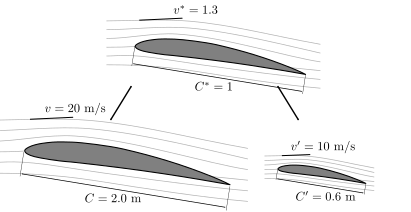
\includegraphics[width=10cm]{../fig/gelijkvormigheid/Dimensieloze_stroomlijnen}
	\end{frame}
%%%%%%%%%%%%%%%%%%%%%%%%%%%%%%%%%%%%%%%%%%%%%%%%%%%%%%%%%%%%%%%%%%%%%%%%%%%
	\begin{frame}
		\frametitle{Dimensieloze getallen}
		\begin{equation}
			\frac{\partial v^*}{\partial t^*} + v^* \frac{\partial v^*}{\partial s^*} =  -\text{Eu} \frac{\partial p^*}{\partial s^*} + \frac{1}{\text{Fr}^2} + \frac{1}{\text{Re}} \frac{\partial^2 v^*}{\partial s^{*2}}
		\end{equation}
		\pause
		\center
		Dimensieloze getallen zijn verhoudingen van referentiewaarden voor krachten
		\pause
		\vspace{0.5cm}
		\begin{alignat*}{3}
			&\text{Re} &&= \dfrac{\rho v D}{\mu} = \dfrac{v D}{\nu} &&= \dfrac{\text{traagheidskracht}}{\text{viskeuze krachten}} \\
			&\text{Eu} &&= \dfrac{p}{\rho v^2} &&= \dfrac{\text{drukkracht}}{\text{traagheidskracht}} \\
			&\text{Fr} &&= \dfrac{v}{\sqrt{g D}} &&= \sqrt{\dfrac{\text{traagheidskracht}}{\text{zwaartekracht}}}
		\end{alignat*}
	\end{frame}
%%%%%%%%%%%%%%%%%%%%%%%%%%%%%%%%%%%%%%%%%%%%%%%%%%%%%%%%%%%%%%%%%%%%%%%%%%%
  	\begin{frame}
		\frametitle{Dimensieloze getallen en gelijkvormigheid}
		\begin{itemize}
			\item<1-3> Gelijke verhoudingen van afstanden
			\item<1-3> Gelijke verhoudingen van snelheden
			\item<2-3> Gelijke verhoudingen van krachten
		\end{itemize}
		\only<2>{
        	\center
        	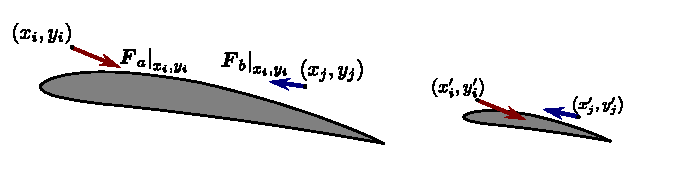
\includegraphics[width=11cm]{../fig/gelijkvormigheid/Gelijkvormigheid_dynamisch}
		}
		\only<3>{
        	\center
        	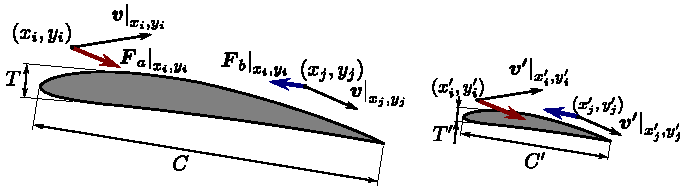
\includegraphics[width=11cm]{../fig/gelijkvormigheid/Gelijkvormigheid}
		}
		\only<3>{
			\begin{equation*}
				\text{Re} = \text{Re'}, \quad \text{Eu} = \text{Eu'}, \quad \text{Fr} = \text{Fr'}
			\end{equation*}
		}
	\end{frame}
%%%%%%%%%%%%%%%%%%%%%%%%%%%%%%%%%%%%%%%%%%%%%%%%%%%%%%%%%%%%%%%%%%%%%%%%%%%
	\begin{frame}
		\frametitle{Dimensieloze getallen}
		\noindent
		\begin{columns}[t,onlytextwidth]
			\column{.25\textwidth}
			\begin{align*}
				\text{Re} &= \dfrac{\rho v D}{\mu} \\
				\text{Eu} &= \dfrac{p}{\rho v^2} \\
				\text{Fr} &= \dfrac{v}{\sqrt{g D}} \\
				\text{Ma} &= \dfrac{v}{c} \\
				\text{St} &= \dfrac{f D}{v}
			\end{align*}
			\column{.30\textwidth}
			\pause
			\begin{align*}
				\text{Pr} &= \dfrac{\nu}{\alpha} \\
				\text{Nu} &= \dfrac{h D}{k} \\
				\text{Gr} &= \dfrac{g \beta (T_s-T_{\infty}) D^3}{\nu^2} \\
				\text{Ra} &= \text{Gr} \text{Pr}
			\end{align*}
			\column{.40\textwidth}
			\pause
			\begin{align*}
				C_p &= \dfrac{p}{\frac{1}{2} \rho v^2} \simeq \dfrac{p}{\rho N^2 D^2} \\
				C_F &= \dfrac{F}{\frac{1}{2} \rho v^2 A} \simeq \dfrac{F}{\frac{1}{2} \rho v^2 D^2} \\
				C_P &= \dfrac{P}{\frac{1}{2} \rho v^3 D^2} \simeq \dfrac{P}{\rho N^3 D^5} \\
				C_{\dot{V}} &= \dfrac{\dot{V}}{v D^2} \simeq \dfrac{\dot{V}}{N D^3}
			\end{align*}
		\end{columns}
	\end{frame}
%%%%%%%%%%%%%%%%%%%%%%%%%%%%%%%%%%%%%%%%%%%%%%%%%%%%%%%%%%%%%%%%%%%%%%%%%%%
	\section{Buckingham-Pi}
	\begin{frame}
		\frametitle{Voorbeeld}
		\begin{textblock}{6}(0,3)
            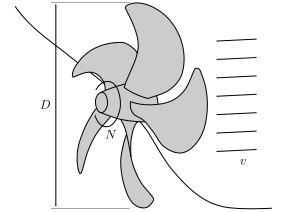
\includegraphics[width=6cm]{../fig/gelijkvormigheid/Dimensieanalyse_voorbeeld_propellor}
        \end{textblock}
        \pause
		\hfill
		\tiny
		\begin{tabular}{lcccc}
			\hline
			Meting  & $N$   & $D$ & $v$   & $F$\\
			        & (rpm) & (m) & (m/s) & (kN)\\
			\hline                          
	        1 & 100 & 0.20 & 2.5 & 1.0 \\       
	        2 & 200 & 0.20 & 2.5 & 1.5 \\       
	        3 & 300 & 0.20 & 2.5 & 1.5 \\       
	        4 & 100 & 0.40 & 2.5 & 4.6 \\       
	        5 & 200 & 0.40 & 2.5 & 4.3 \\       
	        6 & 300 & 0.40 & 2.5 & 2.7 \\       
	        7 & 100 & 0.60 & 2.5 & 9.0 \\       
	        8 & 200 & 0.60 & 2.5 & 3.2 \\       
	        9 & 300 & 0.60 & 2.5 & 0.2 \\       
	        10 & 100 & 0.20 & 5.0 & 1.8 \\      
	        11 & 200 & 0.20 & 5.0 & 3.1 \\      
	        12 & 300 & 0.20 & 5.0 & 4.0 \\      
	        13 & 100 & 0.40 & 5.0 & 8.1 \\      
	        14 & 200 & 0.40 & 5.0 & 11.8 \\     
	        15 & 300 & 0.40 & 5.0 & 11.0 \\     
	        16 & 100 & 0.60 & 5.0 & 19.1 \\     
	        17 & 200 & 0.60 & 5.0 & 19.8 \\     
	        18 & 300 & 0.60 & 5.0 & 14.3 \\     
	        19 & 100 & 0.20 & 7.5 & 2.1 \\      
	        20 & 200 & 0.20 & 7.5 & 3.7 \\      
	        21 & 300 & 0.20 & 7.5 & 5.7 \\      
	        22 & 100 & 0.40 & 7.5 & 10.5 \\     
	        23 & 200 & 0.40 & 7.5 & 17.6 \\     
	        24 & 300 & 0.40 & 7.5 & 22.2 \\     
	        25 & 100 & 0.60 & 7.5 & 23.8 \\     
	        26 & 200 & 0.60 & 7.5 & 41.5 \\     
	        27 & 300 & 0.60 & 7.5 & 34.7 \\                                 
			\hline
		\end{tabular}
	\end{frame}
%%%%%%%%%%%%%%%%%%%%%%%%%%%%%%%%%%%%%%%%%%%%%%%%%%%%%%%%%%%%%%%%%%%%%%%%%%%
	\begin{frame}
		\frametitle{Voorbeeld}
		\center
        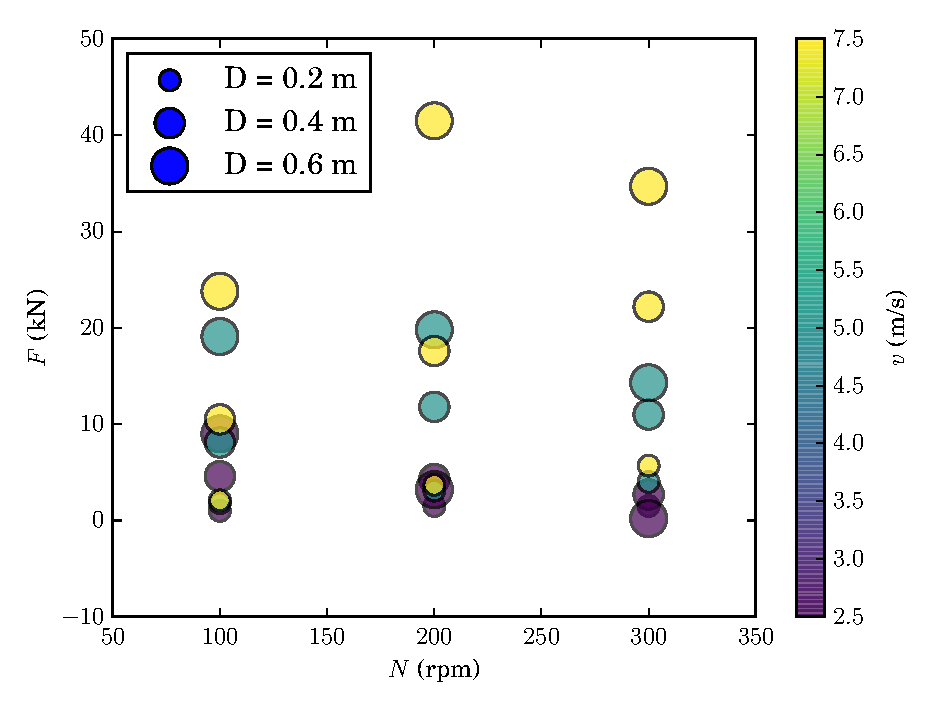
\includegraphics[height=7cm]{../fig/gelijkvormigheid/Dimensieanalyse_voorbeeld_data}
	\end{frame}
%%%%%%%%%%%%%%%%%%%%%%%%%%%%%%%%%%%%%%%%%%%%%%%%%%%%%%%%%%%%%%%%%%%%%%%%%%%
	\begin{frame}
		\frametitle{Eenheden}
		\center
		\begin{tabular}{lll}
			\hline
			Grootheid                   & Dimensie   & Eenheid \\
			\hline
			Lengte                       & \unit{L}                      &   \unit{m} \\
			Massa                        & \unit{M}                      &   \unit{kg} \\
			Tijd                         & \unit{T}                      &   \unit{s} \\
			Dichtheid                    & \unit{ML^{-3}}                &   \unit{kg/m^3} \\
			Druk                         & \unit{ML^{-1}T^{-2}}          &   \unit{N/m^2} \\	
			Dynamische viscositeit       & \unit{MT^{-1}L^{-1}}          &   \unit{Pa s} \\
			Energie (arbeid)             & \unit{ML^{2}T^{-2}}           &   \unit{J} \\
			Impuls                       & \unit{MLT^{-1}}               &   \unit{kg m/s} \\
			Kinematische viscositeit     & \unit{L^{2}T^{-1}}            &   \unit{m^2/s} \\
			Kracht                       & \unit{MLT^{-2}}               &   \unit{N} \\
			Snelheid                     & \unit{LT^{-1}}                &   \unit{m/s} \\
			Vermogen                     & \unit{ML^{2}T^{-3}}           &   \unit{J/s} \\
			Versnelling                  & \unit{LT^{-2}}                &   \unit{m/s^2} \\
			Volume                       & \unit{L^3}                    &   \unit{m^3} \\
			\hline
		\end{tabular}
	\end{frame}
%%%%%%%%%%%%%%%%%%%%%%%%%%%%%%%%%%%%%%%%%%%%%%%%%%%%%%%%%%%%%%%%%%%%%%%%%%%
	\begin{frame}
		\frametitle{Buckingham-Pi theorema}
		\only<1-2>{
			Een relatie:
			\begin{equation*}
				a = f\left( a_1,a_2,\ldots,a_n \right)
			\end{equation*}
			
			met $k$ grootheden met onafhankelijke dimensies
		}
		\only<2-2>{
		
			\vspace{1cm}
			kan herschreven worden als:
			\begin{equation*}
				\pi = f\left( \pi_1,\pi_2,\ldots,\pi_{n-k} \right)
			\end{equation*}
			
			met $\pi, \pi_1,\ldots,\pi_{n-k}$ dimensieloze grootheden
		}
	\end{frame}	
%%%%%%%%%%%%%%%%%%%%%%%%%%%%%%%%%%%%%%%%%%%%%%%%%%%%%%%%%%%%%%%%%%%%%%%%%%%
	\begin{frame}
		\frametitle{Voorbeeld}
		\only<1>{
			\center
        	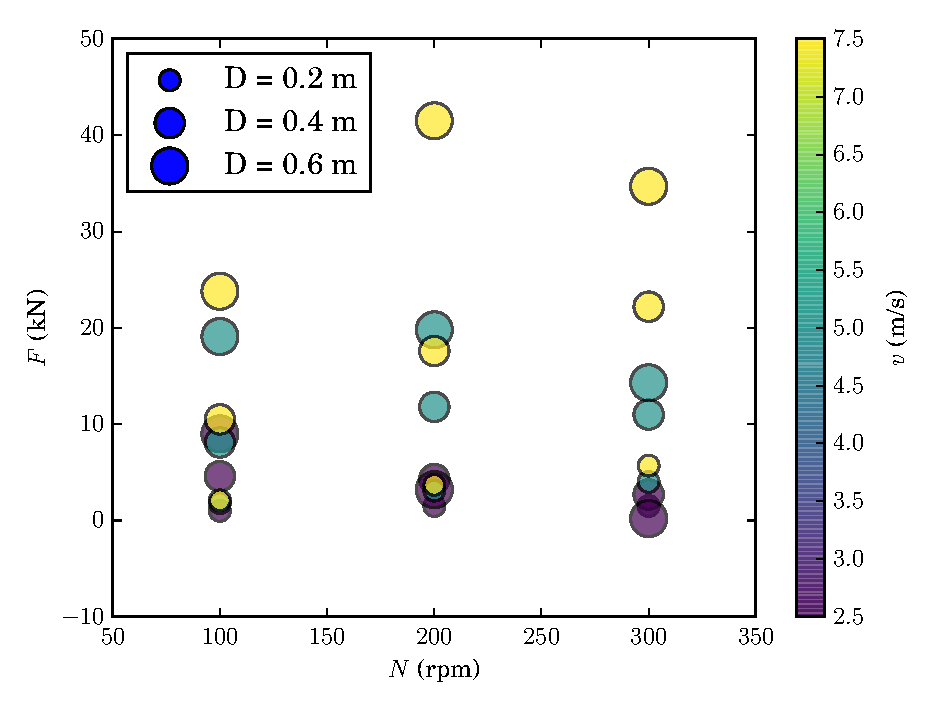
\includegraphics[height=7cm]{../fig/gelijkvormigheid/Dimensieanalyse_voorbeeld_data}
        }
        \only<2>{
        	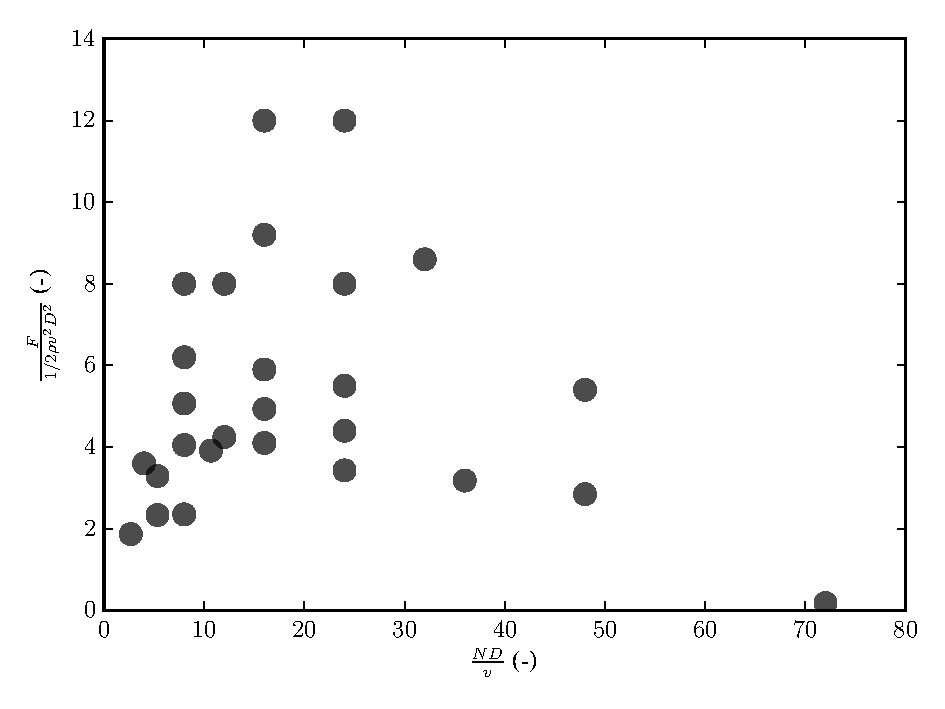
\includegraphics[height=8cm]{../fig/gelijkvormigheid/Dimensieanalyse_voorbeeld_data_dimensieloos_1par}
        }
        \only<3>{
        	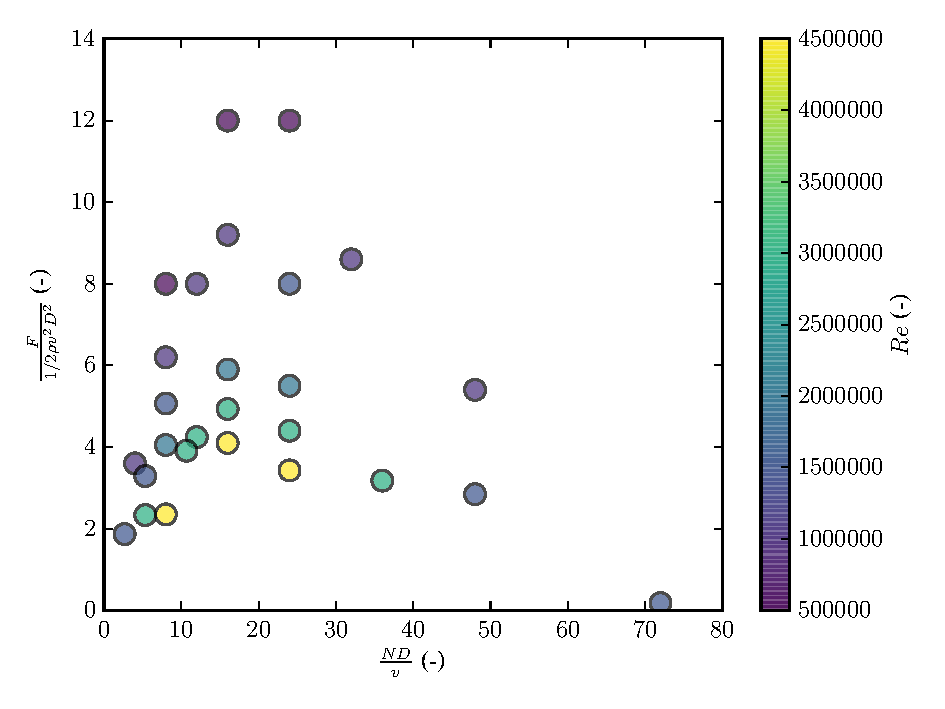
\includegraphics[height=8cm]{../fig/gelijkvormigheid/Dimensieanalyse_voorbeeld_data_dimensieloos}
        }
        \only<4>{
        	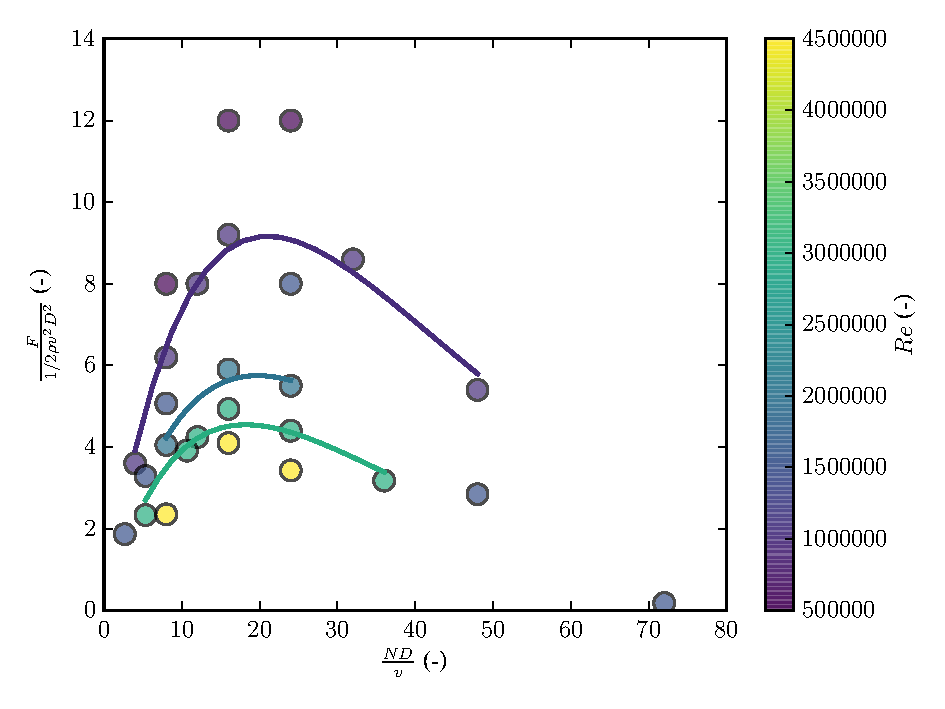
\includegraphics[height=8cm]{../fig/gelijkvormigheid/Dimensieanalyse_voorbeeld_data_dimensieloos_trends}
        }	
	\end{frame}
%%%%%%%%%%%%%%%%%%%%%%%%%%%%%%%%%%%%%%%%%%%%%%%%%%%%%%%%%%%%%%%%%%%%%%%%%%%
\end{document}			